\documentclass{article}
\usepackage[margin=1in]{geometry}
\usepackage{enumitem}
\usepackage{setspace}
\usepackage{amsmath}
\usepackage{amssymb}
\usepackage{physics}
\usepackage{relsize}
\usepackage{graphicx}
\usepackage{multicol}

\title{Math 174E Midterm}
\date{5/7/2021}
\author{Jiaping Zeng}

\begin{document}
\setstretch{1.35}

I certify on my honor that I have neither given nor received any help, or used any non-permitted resources, while completing this evaluation.\\
Signature: 
\includegraphics[width=2in]{signature.png}\\
Date: 5/7/2021
\newpage
\begin{enumerate}
      \item Today's price of the Tesla, Inc. stick is $S_0=\$663$.\\An investor instructs a broker to sell five European put options with maturity July 16, 2021, with a strike price of $K=\$600$ which are currently trading for $\$41$ per option.
            \begin{enumerate}
                  \item Briefly explain what the investor has agreed to.\\
                        \textbf{Answer}: The investor agreed to sell five European put options with strike price $\$600$ that expire on July 16, 2021 for $\$41$ each. Each of these would allow someone to sell a share of Tesla stock on July 16, 2021 for $\$600$.
                  \item Provide the investor's profit and loss on July 16, 2021 (the maturity date $T$) as a function of the then prevailing Tesla stock price $S_T$. Sketch the graph of the function and add suitable annotations.\\
                        \textbf{Answer}: $\$41-(\$600-S_T)^+$;
                        \begin{center}
                              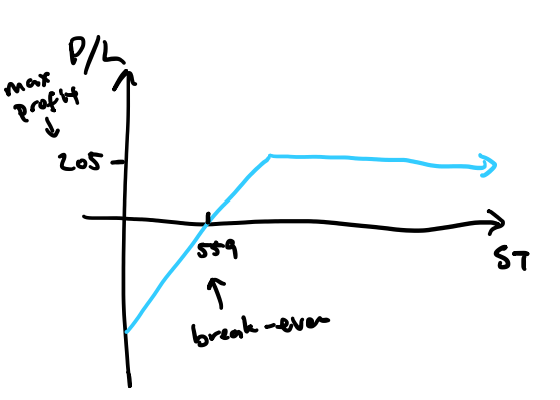
\includegraphics[width=3in]{1c.png}
                        \end{center}
                  \item What must Tesla's stock price $S_T$ at maturity $T$ satisfy so that the trade will be profitable for the investor?\\
                        \textbf{Answer}: The breakeven price is $\$600-\$41=\$559$, so the investor would profit if $S_T>\$559$ and lose if $S_T<\$559$.
                  \item Suppose Tesla's stock price on July 16, 2021 will be either $S_T=\$700$ or $S_T=\$500$, respectively. What is the corresponding P\&L for the investor in both scenarios?\\
                        \textbf{Answer}:
                        \begin{enumerate}
                              \item $S_T=\$700$: $5\cdot\$41=\$205$ profit
                              \item $S_T=\$500$: $5\cdot[\$41-(\$600-\$500)]=-\$295$ loss
                        \end{enumerate}
            \end{enumerate}
            \newpage
      \item Today a company expects to sell 100,000 units of a particular asset A in 6 months in the spot market (on November 15, 2021). The treasurer of the company wishes to hedge the company's exposure to changes in asset A's spot price and decides to use futures contracts on another related asset (with maturity month December 2021). Changes in the spot price of asset A have a 0.80 correlation with changes in the futures price of the related asset. The standard deviation of the spot price changes of asset A is $20\%$ higher than the standard deviation of price changes in the futures prices of the related asset.\\Each futures contract on the related asset is on 10,000 units and the December 2021 futures currently trade at $\$30$ per unit.
            \begin{enumerate}
                  \item If December 2021 futures are used to hedge the exposure, what should the minimum variance hedge ratio be?\\
                        \textbf{Answer}: $h^*=\rho\dfrac{\sigma_S}{\sigma_{\hat{F}}}=0.80\cdot 1.20=0.96$.
                  \item Should the treasurer take a long or short position in the futures contracts? And in how many?\\
                        \textbf{Answer}: Short position; $N^*=\dfrac{h^*\cdot N_A}{Q_{\hat{F}}}=\dfrac{0.96\cdot 100000}{10000}=9.6\approx 10$.
            \end{enumerate}
            Suppose that on November 15, 2021 the spot price of asset A is $\$28$ per unit, and the company closes out its position in the futures contracts at a then prevailing December 2021 futures price of $\$27$.
            \begin{enumerate}[resume]
                  \item What would be the company's total profit and loss from its trade in the futures contract on November 15, 2021 in this scenario?\\
                        \textbf{Answer}: $10\cdot 10000\cdot (\$30-\$27)=\$300000$ profit.
                  \item How much money would the company effectively receive (including its profit or loss from the hedge) to sell the $100,000$ of asset A on November 15, 2021 in the spot market in this scenario?\\
                        \textbf{Answer}: $100000\cdot\$28+\$300000=\$3100000$.
            \end{enumerate}
            \newpage
      \item The following table gives the prices of bonds:
            \[\begin{tabular}{c|c|c|c}
                        Bond principal (\$) & Maturity (years) & Annual coupon (\$) & Bond price (\$) \\
                        \hline
                        100                 & 0.25             & 0.0                & 97.50           \\
                        100                 & 0.50             & 0.0                & 94.90           \\
                        100                 & 1.00             & 0.0                & 90.00           \\
                        100                 & 1.50             & 8.0                & 96.00
                  \end{tabular}\]
            Half the stated coupon is assumed to be paid every six months.
            \begin{enumerate}
                  \item Calculate the zero rates (p.a. and continuously compounded) for all given maturities.\\
                        \textbf{Answer}:
                        \begin{enumerate}
                              \item $n=0.25$: $100e^{-0.25r_0(0.25)}=97.50\implies r_0(0.25)=\dfrac{1}{0.25}\ln\dfrac{100}{97.50}=10.127\%$
                              \item $n=0.5$: $100e^{-0.50r_0(0.50)}=94.90\implies r_0(0.50)=\dfrac{1}{0.50}\ln\dfrac{100}{94.90}=10.469\%$
                              \item $n=1.00$: $100e^{-r_0(1.00)}=90.00\implies r_0(1.00)=\ln\dfrac{100}{90.00}=10.536\%$
                              \item $n=1.50$: $4e^{-0.5r_0(0.5)}+4e^{-r_0(1)}+104e^{-1.5r_0(1.5)}=96.00\implies r_0(1.50)=10.681\%$
                        \end{enumerate}
                  \item Compute the implied forward rate (p.a. and continuously compounded) for the period 12 months to 18 months.\\
                        \textbf{Answer}: $f_0(1,1.5)=\dfrac{1.5r_0(1.5)-1.0r_0(1.0)}{1.5-1.0}=\dfrac{1.5\cdot 10.681\%-10.536\%}{0.5}=10.971\%$.
            \end{enumerate}
            \newpage
      \item Today's value of the S\&P 500 stock index is at 4,200. The stocks underlying the index provide an estimated dividend yield of 1.4\% p.a. (continuously compounded). The risk-free rate is at 1.6\% p.a. (continuously compounded).\\Consider a 5-month forward contract on the S\&P 500 stock index.
            \begin{enumerate}
                  \item Compute today's arbitrage-free forward price of the 5-month forward contract.\\
                        \textbf{Answer}: $F=Se^{(r-q)T}=4200e^{(0.016-0.014)\cdot\frac{5}{12}}=4200e^{\frac{0.010}{12}}=\$4203.501458$.
            \end{enumerate}
            Suppose you are entering today into a short position in the 5-month forawrd contract on the S\&P 500 with the forward price computed in (a).
            \begin{enumerate}[resume]
                  \item What is the value of this short position in the forward contract today?\\
                        \textbf{Answer}: $0$ since all forward contracts have initial value of $0$.
                  \item Assume in two months the S\&P 500 index will be at 4,100. What will be the value of your short position in the forward contract then?\\
                        \textbf{Answer}: $f_t=Se^{(r-q)T}-S_T=4200e^{(0.016-0.014)\cdot\frac{2}{12}}-4100=\$101.400233$.
            \end{enumerate}
            \newpage
      \item Companies A and B have been offered the following rates per annum on a $\$50$ million five-year loan:
            \[
                  \begin{tabular}{c|c|c}
                                  & fixed rate & floating rate \\
                        \hline
                        Company A & 12.0\%     & LIBOR         \\
                        Copmany B & 13.4\%     & LIBOR + 0.5\%
                  \end{tabular}
            \]
            Company A requires a floating-rate loan, whereas company B needs a fixed-rate loan.
            \begin{enumerate}
                  \item Design a swap contract with an investment bank acting as an intermediary (which takes $0.1\%$) and that is equally attractive to both companies.\\
                        \textbf{Answer}: We have Company A borrow at fixed rate $12.0\%$ and Company B borrow at floating rate LIBOR + $0.5\%$, then enter a swap to convert the liability (fixed to floating for Company A and floating to fixed for Company B).
                  \item What is the total gain for both companies with the swap contract? What is the net gain for company A and what is the net gain for company B?\\
                        \textbf{Answer}: Total gain is $(13.4\%-12.0\%)-0.5\%-0.1\%=0.8\%$, so the net gains for both companies are $\dfrac{0.8\%}{2}=0.4\%$.
            \end{enumerate}
\end{enumerate}

\end{document}